\chapter{Level Set Methods}
A level set formulation is an implicit representation of a closed curve or curves. 
The curve is represented as a constant value of a higher dimensional function.
A familiar example of such level curves are level curves on a map. Provided 
a continuous function of the elevation of the ground surface on an area, the level
contours joins points on the surface of equal elevation. All curves representing the 
same value, or elevation in the cartographic setting, are called \textit{iso-curves} or
\textit{iso-contours}. On a map, there are numerous iso-curves of different values 
separated by a constant height. Such contours are thus effectively describing
the steepness and height, and thus the shape, of the ground in the area. 
In a level set context, we are not interested in the shape of the underlying 
higher dimensional function. We look at a single iso-value and the standard 
practice is to use the zero iso-value. The corresponding curve(s) will 
split the domain into regions of two types. One where the underlying function is 
positive, and one where it is negative. In contrast to cartography, level set 
methods only tracks the shape of the surfaces of these regions and how they 
change over time.

\todo{cool: image of a function that is cut at a specific value}

\begin{comment}
To continue with the cartographic image, 
The image of contours on a map is useful when understanding iso-curves in a
level set setting also. Since the level set formulation is a way of describing
closed curves, we need to know under which circumstances iso-contours forms 
closed curves. As we are used to from maps, elevation curves are always closed.
\todo{Fullfør. Kontinuitet?}
\end{comment}

\newpage
\section{Level Set Definition}
Now that we have an intuition about iso-curves, we can discuss the principle
of a level set method. The goal is to represent a closed curve or surface, 
$\Gamma(t)$, that moves under the influence of a velocity field $\vv{v}$.
The level set approach to this problem, as first presented in 1987 by 
S.Osher and J. Sethian \cite{Osher-Sethian}, is to define a continuous function
\uxt defined on a domain \domain containing $\Gamma|_{t=0}$.
The domain \domain is split in two parts by the curve $\Gamma$, the interior
$\Omega$ and the exterior \domain $\setminus \Omega$. 
\begin{figure}
    \centering
    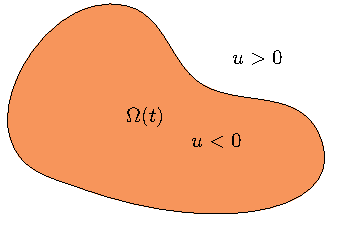
\includegraphics[width=.5\linewidth]{figures/tikz-figures/optimization-problem.pdf}
    \caption{Level set representation of a curve $\Gamma (t)$.}
    \label{fig:levelset-representation}
\end{figure}
The function \uxt must be constructed in a way that it satisfies the following properties
\begin{align}
    u(\mathbf{x}, t) < 0 \qquad &\text{for } \mathbf{x} \in  \Omega(t) \label{eq:interior}\\
    u(\mathbf{x}, t) = 0 \qquad &\text{for } \mathbf{x} \in  \Gamma(t) \label{eq:zero-iso-curve}\\
    u(\mathbf{x}, t) > 0 \qquad &\text{for } \mathbf{x} \in  \mathcal{D} \setminus \Omega(t) \label{eq:exterior}.
\end{align}
Now, the curve $\Gamma$ can be described in terms of \uxt by being its 
zero iso-contour. This means that if we can find the proper evolution of 
\uxt we can implicitly track the motion of the curve $\Gamma$.
Now, what we need is to find a model for the change in \uxt in order
to simulate the level curve $\Gamma$ as a curve flowing in the velocity field $\vv{v}$.
Because the zero iso-curve of \uxt is the only region of interest, we differentiate 
\eqref{eq:zero-iso-curve} with respect to time in order to find how the function \uxt
changes over time at the curve, $\Gamma$. 
\begin{equation}
    (u(\mathbf{x}, t)_t + \nabla u(\mathbf{x}, t) \, \Gamma_t)_{\mathbf{x}\in \Gamma} = 0
    \label{eq:general-u-flow}
\end{equation}
When $\Gamma$ flows in the velocity field $\vv{v}$, its time derivative has to be 
defined as \todo{dette er ikke helt bra:}
\begin{equation}
    \Gamma_t = \vv{v}\cdot \vv{n}_{\Gamma} = v_n \vv{n}_{\Gamma}.
\end{equation}
In addition, we can see from \eqref{eq:interior}-\eqref{eq:exterior} that the gradient 
of $u$ at the curve $\Gamma$ is always pointing in the direction of the normal vector of 
$\Gamma$, $\vv{n}_{\Gamma}$. Thus we can write 
\begin{equation}
    \vv{n}_{\Gamma} = -\frac{\nabla u}{|\nabla u|}
\end{equation}

Inserting everything back into \eqref{eq:general-u-flow}, we get the equation
\begin{equation}
    u_t - v_n\, |\nabla u| = 0
    \label{eq:general-level-set}
\end{equation}

We constructed this partial differential equation to let the curve, $\Gamma$, flow in 
our velocity field $\vv{v}$, and the motion of the rest of the higher dimensional curve
\uxt is of less interest. We do see that we could have done exactly the same for 
any other iso-value of \uxt by defining 
\begin{align}
    u(\mathbf{x}, t) < v \qquad &\text{for } \mathbf{x} \in  \Omega_v(t) \label{eq:v-interior}\\
    u(\mathbf{x}, t) = v \qquad &\text{for } \mathbf{x} \in  \Gamma_v(t) \label{eq:v-iso-curve}\\
    u(\mathbf{x}, t) > v \qquad &\text{for } \mathbf{x} \in  \mathcal{D} \setminus \Omega_v(t) \label{eq:v-exterior}.
\end{align}
and differentiated \eqref{eq:v-iso-curve} with respect to time. Because the right hand 
side $v$ is only a constant, this would make no difference to the resulting PDE. Thus
it is not only the zero iso-contour, but the entire function \uxt that is transported 
in the velocity field $\vv{v}$.

We have now found a way to model a curve influenced by a velocity field. Given that 
a proper velocity field exists to transport an arbitrary initial curve, $\Gamma_0$,
into the desired curve $\Gamma_f$ described in \todo{insert}, solving the PDE defined
in \eqref{eq:general-level-set} will yield the desired solution. But there exists other
methods for solving such problems \todo{more}. It is thus appropriate to ask whether 
level set methods are really a good choice. 




What to discuss around the method?
\begin{enumerate}
    \item increased complexity for solving PDE on entire domain. How to fix
    \item Topological flexibility. Situations that are now easily handled.
    \item Existence of viscosity solution (?????). In that case, I must read.
    \item Existence and uniqueness
\end{enumerate}

\newpage
\section{Modelling a choices}
Above, a general level set method is described. Then we had a zero level curve flowing in an unspecified velocity field, \velocityfield. We have shown that, given such velocity field, the PDE in \eqref{eq:general-level-set} will describe the motion of our curve influenced by the field, \velocityfield. Now, in order to obtain a model such as described in \chapref{chap:introduction}, we need to define the right velocity field for our situation.

Our problem can be understood and formulated as a minimization problem. We can construct a fictive potential field or energy function which will give the surface an energy depending on the distance to the point set and curvature. Then we find the speed and direction for the surface, $\Gamma$, to move such that this energy is minimized. This is called \textit{gradient flow}. Gradient flow is in short a continuous gradient descent formulation, such that the motion of a point is always in the direction of maximum descent. For points $\mathbf{x}$ in a domain \domain in a potential field $f(\mathbf{x})$, this can be formulated as:

\begin{equation}
    \mathbf{x}_t = -\nabla f(\mathbf{x}).
    \label{eq:grad-flow}
\end{equation}

Defining the function $f(\mathbf{x})$ is a modeling question and will decide the behavior of our partial differential equation \eqref{eq:general-level-set}. We have to construct the function such that the velocity field moves the surface to the stationary result $\Gamma_f$ that meets our requirements. In order to do this, we must clearly define what those are.

\begin{proposition}[Problem definition]
We want to construct a surface $\Gamma_f$ dependent on the point set $V$ that 
\end{proposition}

provide a velocity field that again will lead our curve to the desired stationary solution $\Gamma_f$. The stationary solution is obtained when $u_t = 0$ which means that the gradient of the potential field is zero, as seen in \eqref{eq:grad-flow}. 

Using our implicit level set formulation of our surface, defined in \eqref{eq:interior}-\eqref{eq:exterior}, we define a potential value function for a domain $\Omega$ as defined in \eqref{eq:interior}. 

\begin{comment}

We now want to use a level set method to solve a problem as described in the
introduction. We have sampled data from an unknown surface/curve and want to
reconstruct the original surface. We then want to find the appropriate velocity
field from \eqref{eq:general-level-set} in a way such that our surface $\Gamma$ 
flows in the direction of our points at the same time as it preserves smoothness. We
approach this by formulating the situation as an optimization problem, or more
specifically, we construct a \textit{gradient flow equation} for our domain $\Omega$. 

Gradient flow is the continuous version of the steepest descent algorithm. The descent methods are optimisation algorithms for finding minimizers of functionals and the idea is
to always move in the direction of steepest descent. Mathematically this is formulated as follows. \todo{define variables} 


In order to use this optimization formulation, we need to construct a function depending
on the domain $\Omega$ that has a minima when, $\Gamma$, the surface of $\Omega$
is the desired surface we are looking for. As we are introducing the movement of $\Gamma$
as a flow, it fits nicely to call this function we are optimizing, an energy function. 
Using that, we can think of our curve moving in a type of gravitational field, drawn
towards the point set V and influenced by a surface tension to ensure smoothness. 

The energy function is only a tool to ensure that the surface, $\Gamma$, flows towards the
desired stationary solution, so the function could be described in numerous ways as long 
as a minima is obtained at our desired curve. However, some functions are more fit than others, as we want hopefully the global minima at the curve and ...    

We would like to move the curve, which is equivalent to changing the interior 
$\Omega$ , such that we minimise the energy functionals defined above \todo{Ikke gjort}. 

* Minimise the functionals we find above. 

* Define our new PDE with the new velocity field. Discuss terms and parameters.

* Local and global minima of the optimisation problem. Integral over domain = Ø is zero. To have a global min on the curve, we need the interior to be negative.

* From the optimisation formulation, we will find the minima which will
be equivalent to finding the stationary solution for our curve. NB: This could not be
the global stationary solution. The velocity will be zero only on the curve. Thus 
we need a stopping criterion for the problem \eqref{eq:general-level-set}. 

\section{Existence of a stationary solution}
\end{comment}

\section{Distance Functions}\label{sec:distance-function}

Distance functions are important for level set methods in general, but they are particularly important for this application. That is because the distance function is a part of the velocity field that drives the surface to our point set.

\begin{definition}
A \textit{distance function}, is the minimal euclidean distance from all points to a point set $\mathcal{V}$. Thus $d(\mathbf{x})$ is defined as 
\begin{equation}
    d(\mathbf{x};\mathcal{V}) = \min_{\mathbf{x}_{v} \in \mathcal{V}} \|\mathbf{x}-\mathbf{x}_{v} \|_2
    \label{eq:unsigned-distance-function}
\end{equation}
\end{definition}

The norm $\|\mathbf{x}-\mathbf{x}_{v} \|$ is positive for all input $\mathbf{x}$ and $\mathbf{x}_{v}$, and thus the distance function is always positive, or \textit{unsigned}.

\todo{Insert proof of $|\nabla d| = 1$?}

The distance function can be the computed to an arbitrary point set, and the notion of a distance function makes intuitively sense. Solving the minimization problem can be time consuming, but as long as $\mathcal{V}\neq \emptyset$, $d(\mathbf{x})$ is uniquely defined everywhere.

The distance function can also be used to measure the distance to a curve. In these cases, one can construct a distance function which in addition displays which regions are inside and outside the curve, by adding a sign. Such a \textit{signed distance function} can thus implicitly describe a curve $\Gamma$ by its zero iso-contour and simultaneously provide information about how every point in the domain relates to the curve $\Gamma$.

\begin{definition}
In a domain \domain including a closed region $\Omega$ with surface $\Gamma$, the signed distance function $u_d$ is defined as
\begin{equation}u_d(\mathbf{x}) = \begin{cases} \, d(\mathbf{x}) \qquad & \text{if } \mathbf{x}\in \Omega\\ -d(\mathbf{x}) \qquad & \text{if } \mathbf{x}\in \mathcal{D} \setminus \Omega\end{cases}
\end{equation}
\end{definition}

In one dimension, this is easily 

